\documentclass[../Cours.tex]{subfiles}

\usepackage{xstring}
\usepackage{xfp}

\begin{document}
\clearpage
\thispagestyle{empty}

\setcounter{DS}{2}

\color{black}
\nomPrenom
\titreDScorrection

\begin{questions}
    \EXERCICETITRE{6}{Symétries}
    \begin{center}
        \begin{tikzpicture}
            \draw (0,0) rectangle (3,2);
            \node[left] at (0,0) {$A$};
            \node[right] at (3,0) {$B$};
            \node[right] at (3,2) {$C$};
            \node[below right] at (0,2) {$D$};
            \draw[dashed] (0,0) -- (3,2);
            \draw (-3,0) -- (3,4);
            \draw (-1.85,2.77) node[left]{$A'$} -- (-0.69,5.54) node[above]{$B'$} -- (1.15,4.77) node[right]{$C'$} -- (0,2) node[above]{$D'$} -- cycle;
        \end{tikzpicture}
        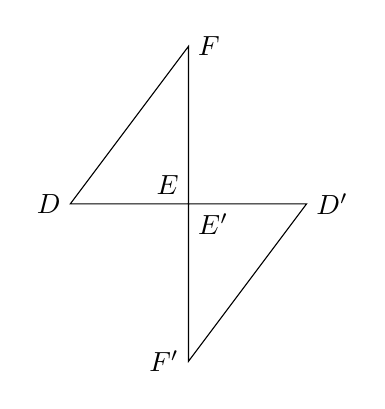
\begin{tikzpicture}[scale=0.5]
            \draw (0,0) node[left]{$D$} -- (3,0) node[above left]{$E$} -- (3,4) node[right]{$F$} -- cycle;
            \draw (3,0) node[below right]{$E'$} -- (6,0) node[right]{$D'$} -- (3,-4) node[left]{$F'$} -- cycle;             
        \end{tikzpicture}
    \end{center}
    
    \EXERCICETITRE{4}{Boite de conserve}
    \question On utilise la formule donnée dans l'énoncé en remplaçant $r$ par \qty{4.95}{\centi\metre} et $h$ par \qty{11.8}{\centi\metre}.

    \begin{align*}
        V_{\mbox{cylindre}} &= \pi \times r \times r \times h \\
        &= \pi \times \qty{4.95}{\centi\metre} \times \qty{4.95}{\centi\metre} \times \qty{11.8}{\centi\metre} \\
        &\approx \qty{908.33}{\centi\metre\cubed}
    \end{align*}

    \question\\
    On sait que $\qty{1000}{\centi\metre\cubed} = \qty{1}{\deci\metre\cubed}$, d'où $\qty{908.33}{\centi\metre\cubed} = \qty{0.90833}{\deci\metre\cubed}$.\\
    Ensuite $\qty{1}{\deci\metre\cubed} = \qty{1}{\litre}$, donc $\qty{0.90833}{\deci\metre\cubed} = \qty{0.90833}{\litre}$.\\
    Enfin $\qty{1}{\litre} = \qty{100}{\centi\litre}$ donc $\qty{0.90833}{\litre} = \qty{90.833}{\centi\litre}$.    

    \EXERCICETITRE{4}{Téléviseurs}
    La plupart des téléviseurs dans le commerce sont au format 16:9, ce qui signifie que la longueur et la largeur du téléviseur sont dans le ratio 16:9.

    \question 
    On peut traduire ce ratio par un tableau de proportionnalité : 
    \begin{center}
        \begin{tabularx}{0.5\linewidth}{|l|C|C|}
            \multicolumn{1}{c|}{} & longueur & largeur \\\hline
            taille (en \unit{\centi\metre}) & 32 & ? \\\hline
            ratio & 16 & 9 \\\hline
        \end{tabularx}
    \end{center}

    En faisant un produit en croix, on obtient : $\dfrac{32 \times 9 }{16} = \qty{18}{\centi\metre}$.

    \question 
    On peut traduire ce ratio par un tableau de proportionnalité : 
    \begin{center}
        \begin{tabularx}{0.5\linewidth}{|l|C|C|}
            \multicolumn{1}{c|}{} & longueur & largeur \\\hline
            taille (en \unit{\centi\metre}) & ? & 45 \\\hline
            ratio & 16 & 9 \\\hline
        \end{tabularx}
    \end{center}

    En faisant un produit en croix, on obtient : $\dfrac{45 \times 16 }{9} = \qty{80}{\centi\metre}$.

    \question Un téléviseur s'apparente à un rectangle, donc : 
    $$\mbox{périmètre} = 2 \times \mbox{longueur} + 2 \times \mbox{largeur} = 250$$
    Cela signifie que : 
    \begin{align*}
        &\mbox{longueur} + \mbox{largeur} = 125 \\
        et& \\
        &\mbox{la longueur et la largeur sont dans le ratio 16:9}
    \end{align*}

    On peut traduire cela par un tableau de proportionnalité : 
    \begin{center}
        \begin{tabularx}{0.5\linewidth}{|l|C|C|C|}
            \multicolumn{1}{c|}{} & longueur & largeur & total \\\hline
            taille (en \unit{\centi\metre}) & ? & ? & 125 \\\hline
            ratio & 16 & 9 & 25\\\hline
        \end{tabularx}
    \end{center}

    Dans ce tableau, pour passer de la ligne du bas à la ligne du haut, on multiplie par 5. On en déduit que la longueur est $16 \times 5 = \qty{80}{\centi\metre}$ et que la largeur est $9 \times 5 = \qty{45}{\centi\metre}$.

    \EXERCICETITRE{4}{Eau salée}
    Pour faire cuire des pâtes, on les introduit dans l'eau bouillante quelques minutes. Il est recommandé d'utiliser \qty{10}{\gram} de sel pour \qty{1}{\kilo\gram} d'eau. On rappelle

    \question Si on utilise \qty{2.7}{\kilo\gram} d'eau, combien de sel doit-on utiliser ?
    \question Si on a utilisé \qty{2}{\gram} de sel, quel quantité d'eau faut-t-il faire bouillir ?

    \question 
    Traduisons cela par un tableau de proportionnalité : 
    \begin{center}
        \begin{tabularx}{0.5\linewidth}{|l|C|C|}
            eau (en \unit{\kilo\gram}) & 1 & \num{2.7} \\\hline
            sel (en \unit{\gram}) & 10 & ? \\\hline
        \end{tabularx}
    \end{center}

    On remarque que pour passer de la première ligne à la deuxième, on multiplie par 10. Cela nous permet de dire que la réponse ici est : $\num{2.7} \times 10 = \qty{27}{\gram}$ de sel.

    \question 
    Traduisons cela par un tableau de proportionnalité : 
    \begin{center}
        \begin{tabularx}{0.5\linewidth}{|l|C|C|}
            eau (en \unit{\kilo\gram}) & 1 & ? \\\hline
            sel (en \unit{\gram}) & 10 & 2 \\\hline
        \end{tabularx}
    \end{center}

    On remarque que pour passer de la deuxième ligne à la première, on divise par 10. Cela nous permet de dire que la réponse ici est : $\num{2} \div 10 = \qty{0.2}{\kilo\gram}$ d'eau.

    \EXERCICETITRE{2}{Multiples et diviseurs}

    \question 
    \begin{align*}
        110 &= 11 \times 10 \\
        &= 11 \times 2 \times 5 \\
        &= 2 \times 5 \times 11 ~~~~~~(\mbox{remis dans l'ordre croissant})\\
    \end{align*}

    Donc les diviseurs de 110 sont : \{ 1, 110, 2, 5, 11, 10, 22, 55 \}
        
    
\end{questions}
\end{document}